\section{Introduction}

\begin{figure*}[t]
\begin{center}
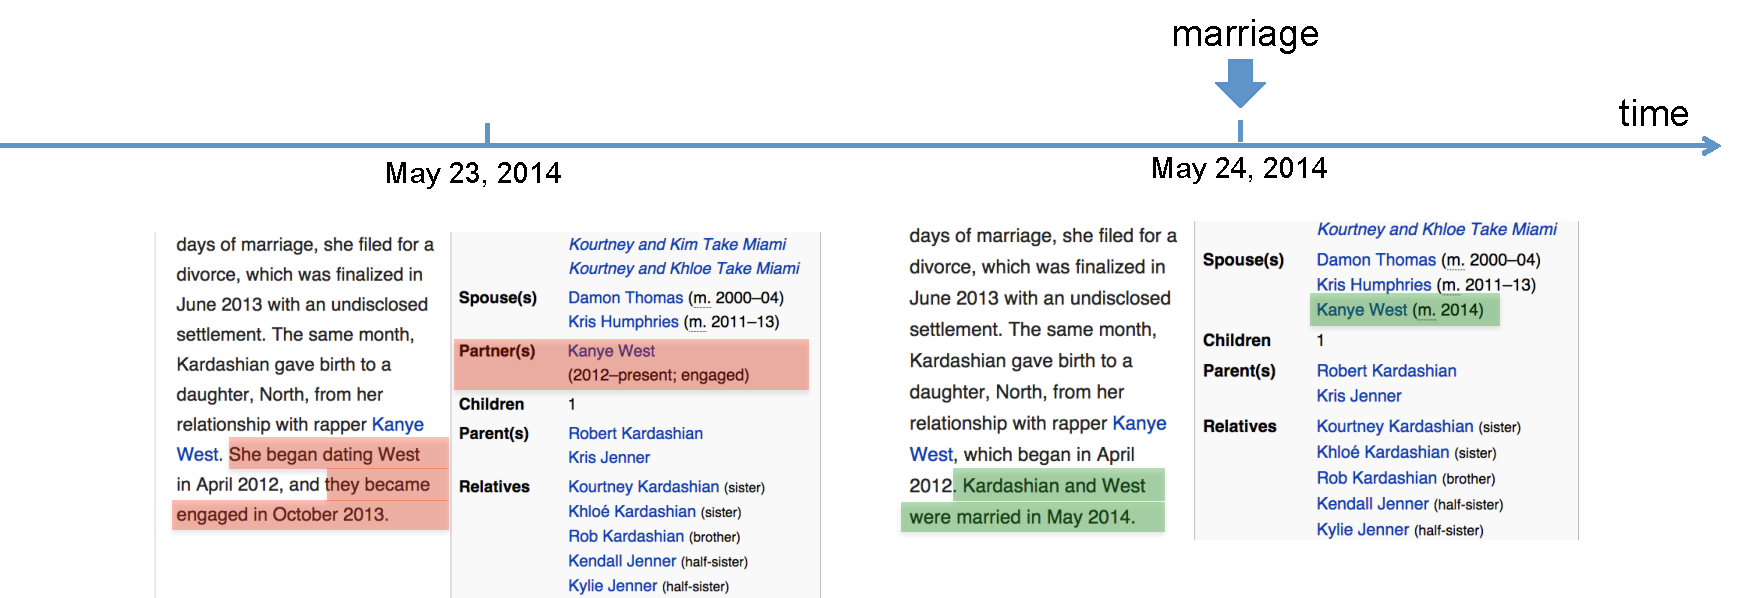
\includegraphics[width=16cm,keepaspectratio=true]{figures/motivation.pdf}
\caption{\label{fig:motivation} A snapshot of Kim Kardashian's Wikipedia revision history, highlighting text and infobox changes. In red (and green) are the differences between the page on 05/25/2014 and 05/23/2014: things that are deleted from (and  added to) the page.}
\end{center}
\end{figure*}

Extracting relational facts between entities and storing them in knowledge bases (KBs) has been a topic of active research in recent years . The resulting  KBs  are generally static  and are not updated as the facts change.  \cite{suchanek2007yago,carlson2010toward,fader2011identifying,MitchellCHTBCMG15}
%(which extract facts from Wikipedia infoboxes \cite{suchanek2007yago}) or NELL (which extracts facts from any Web text \cite{carlson2010toward,fader2011identifying}) are generally static.
 %They are not updated as the Web changes.
 % when in reality new facts arise while others cease to be valid%or change over time
One possible approach to   updating KBs is to extract facts from dynamic Web content such as news \cite{nakashole2012real}. 
In this  paper, we propose to predict state changes caused by  verbs acting on entities in text. This is different from simply applying the same text extraction pipeline, that created the original KB, to dynamic Web content.
%a \textit{shift} of focus from doing KB updates by extracting facts in text to doing them by 

In particular,  our approach has the following advantages: (1) Consider for example the \textsc{spouse} relation, both \textit{marry} and \textit{divorce} are good patterns for extracting this relation. In our work, we wish to learn that they cause different state changes.
%Ndapa: I think most people know this, so we can skip it to keep the text concise
% \textit{marry} signals the start while \textit{divorce} signals the end of the \textsc{spouse} relation; 
Thus,  we can update the entity's fact \textit{and} its temporal scope \cite{wijayactp}. (2) Learning state changing verbs
 %  about by verbs 
   can pave ways for learning the ordering of verbs in terms of their  pre- and post-conditions.
   
   % %Ndapa:
  % I think we are being too speculative here. This was fine in a vision paper such as AKBC but here
  % it might seem like over promising. It is therefore better to not ay much here. 
  
   % of state-changing verbs: the entry condition (in terms of KB facts) that must be true for an event expressed by the verb to take place, and the exit condition (in terms of KB facts) that will be true after the event. Such pre- and post-conditions can be useful for (a) learning event sequences %such as scripts \cite{schank2013scripts}, which can be modeled
%as a collection of verbs chained together by pre- and post-condition of their shared entities, (b) for inferring cascading effect of an event via the pre- and post-condition of shared entities in an event sequence, or (c) for inferring unknown states of entities from the verbs they participate in.  

Our approach learns state changing verbs from Wikipedia revision history. In particular, we seek to establish a correspondence between infobox edits and verbs edits in the same article. The infobox of a  Wikipedia article is  a structured box that summarizes an entity as a set of facts (attribute-value pairs) . Our assumption is that when a state-changing event happens to an entity e.g., a marriage, its Wikipedia infobox is  updated by adding a new \textsc{spouse} value. 
At the same time, the article text  might be updated with verbs that express the event, e.g., \textit{X is now \textbf{married} to Y}.  Figure \ref{fig:motivation} is an example of an infobox of entity changing at the same time as the article's main text to reflect an marriage event.

Wikipedia revision history of many articles can act as distant supervision  data for learning the correspondence between text and infobox changes. However, these revisions are very  \textit{noisy}.  Many infobox slots can be  updated when a single event happens.
%there is no guarantee that only the infobox slots related to a particular event will be updated. 
For example, when a death happens, slots regarding birth e.g., \textit{birthdate}, \textit{birthplace}, may also be updated or added if they were missing before.
Therefore, our method has to handle these sources of noise.  We leverage logical constraints  to rule out meaningless mappings  between infobox and text changes. 
% e.g., that the start of \textit{deathdate} is mutually exclusive from the \textit{birthdate} or that the start of \textit{birthdate} is simultaneous with the start of \textit{birthplace}.
%to effectively learn infobox changes that relate to a particular event-expressing verb. 

<<<<<<< HEAD
In summary, our contributions are as follows: (1) the preparation and use of  distantly labeled dataset curated from Wikipedia revision history for learning state changes, which we make available for future research\footnote{URL retracted for blind reviews},(2) a resource of verbs for identifying state changes, which we also make available, and (3) showing that unstructured text changes in Wikipedia can be used to predict updates to the semi-structured infoboxes. 
=======
In summary, our contributions are as follows: (1) We  extracted a  distantly labeled dataset from Wikipedia revision history targeted for the task of  learning verbs that cause  infobox updates, which we showed to be effective for learning state changing verbs.  (2) We developed a method for learning state changing verbs from Wikipedia revision history.
(3) A resource that contains state changing verbs, which we make available for future research \footnote{URL retracted for blind reviews}. We also make the revision history dataset available.
>>>>>>> upstream/master
% learned resource of verbs that is effective for identifying state changes\footnote[1]{We make our dataset and verbs resource available here: http://.../verbs.html}.